\documentclass{article}

\usepackage[margin=0mm, paperwidth=94.5mm, paperheight=72.4mm]{geometry}

\usepackage{tikz}
\usetikzlibrary{bayesnet}

\begin{document}
\thispagestyle{empty}

\begin{center}
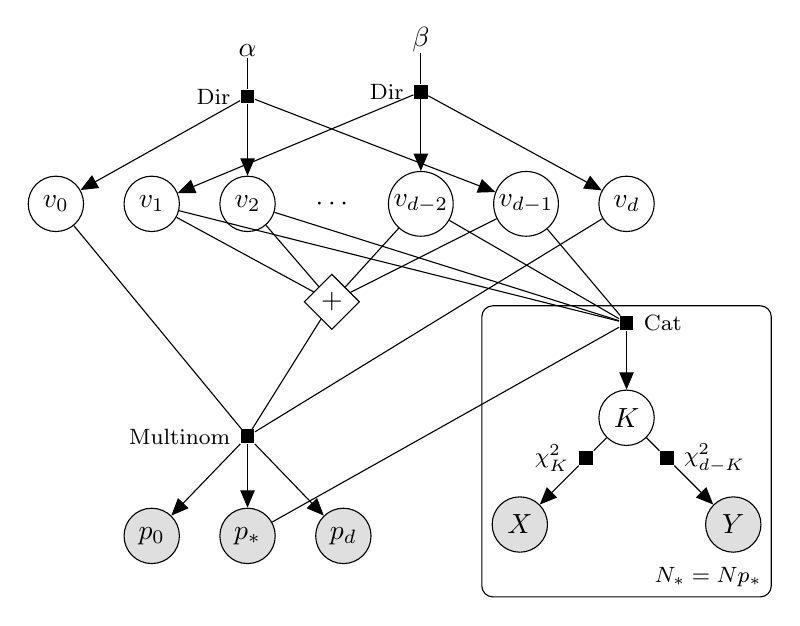
\begin{tikzpicture}
   \node[det] (sum) {$+$} ;
   \node[const, above=.8 of sum] (vdots) {$\cdots$} ;
   \node[latent, left=.5 of vdots] (v2) {$v_2$} ;
   \node[latent, left=.5 of v2] (v1) {$v_1$} ;
   \node[latent, left=.5 of v1] (v0) {$v_0$} ;
   \node[latent, right=.5 of vdots] (vdm2) {$v_{d-2}$} ;
   \node[latent, right=.5 of vdm2] (vdm1) {$v_{d-1}$} ;
   \node[latent, right=.5 of vdm1] (vd) {$v_d$} ;
   
   \node[const, above=1.5 of v2] (alpha) {$\alpha$} ;
   \node[const, above=1.5 of vdm2] (beta) {$\beta$} ;
   \factor[below=of alpha] {alp-f} {left:Dir} {alpha} {v0,v2,vdm1} ;
   \factor[below=of beta] {bet-f} {left:Dir} {beta} {v1,vdm2,vd} ;

   \edge[-] {v1,v2,vdm2,vdm1} {sum} ;
   
   \node[obs, below=3.5 of v2] (bulk) {$p_*$} ;
   \node[obs, left=.5 of bulk] (p0) {$p_0$} ;
   \node[obs, right=.5 of bulk] (pd) {$p_d$} ;
   \factor[below=2.5 of v2] {extr-f} {left:Multinom} {v0,sum,vd} {bulk,p0,pd} ;
   
   \node[latent, below=2 of vd] (K) {$K$} ;
   \node[obs, below left=1.2 of K] (X) {$X$} ;
   \node[obs, below right=1.2 of K] (Y) {$Y$} ;
   \factor[above right=.7 of X] {X-f} {left:$\chi_K^2$} {K} {X} ;
   \factor[above left=.7 of Y] {Y-f} {right:$\chi_{d-K}^2$} {K} {Y} ;
   \factor[above=.75 of K] {K-f} {right:Cat} {bulk,v1,v2,vdm2,vdm1} {K} ;

   \plate {KXY} {(K)(K-f)(X)(Y)} {$N_*=Np_*$} ;
\end{tikzpicture}
\end{center}

\end{document}











